\section{From calibrated comparisons to selected procedures}
\label{sec:conference-experiments}

The experiments ask which effects remain when we change the comparison
protocol. We distinguish three settings: exact fresh-sample moments,
replacement SGD on sampled noisy training sets, and held-out evaluation
on a fixed categorical dataset. An observation budget counts every sampled
training row, including repeated visits. All results below concern final
iterates selected from stored checkpoints.

\subsection{Rate and stopping adjustments}

A follow-up exact-moment study covers 228 binary laws, 51,048 training
configurations, and 2,571,800 endpoints. It varies prevalence, dependence,
signal, noise, rates, batches, and stopping, and retains fixed-update and
fixed-observation comparisons. The primary adjusted comparison selects
the lowest exact risk among mean-square stable configurations and
initialization. It uses a coarse rate range from $1.953125\times10^{-6}$
to $.64$, with a separate resolution check on 16 laws. This is oracle
selection with a known test law, not validation selection.

Both original anchor comparisons disappear after the declared adjustments.
For the independent anchor of Theorem~\ref{thm:conference-c1},
Table~\ref{tab:conference-adjustment} reports the rare-risk gap at the
fixed configuration and after rate/stopping selection. The late $B=1$
disadvantage for S disappears; the selected rates are $h_U=.004$ and
$h_S=.0003125$. At the dependent anchor of
Theorem~\ref{thm:conference-c2}, adjusted selection favors U under both
objectives. Other laws retain reversals or produce objective disagreement.
The theorems therefore describe a calibrated procedure, while the search
answers a different question about the available family of procedures.

\begin{table}[t]
\centering
\begin{tabular}{rrrr}
\toprule
$B$ & $k$ (cap) & Fixed gap & Adjusted gap \\
\midrule
1 & 1,000 & $-.266270$ & $-.005695$ \\
1 & 10,000 & $+.050643$ & $-.002562$ \\
10 & 1,000 & $-.334899$ & $-.001381$ \\
10 & 10,000 & $-.014046$ & $-.000103$ \\
\bottomrule
\end{tabular}
\caption{SD-minus-U rare risk at the independent anchor. Adjusted gaps
use the declared coarse stable oracle search at the same observation cap.
The original stopping reversal disappears under this search.}
\label{tab:conference-adjustment}
\end{table}

The study retains invalid candidates in unrestricted reports rather than
silently removing them. Some unrestricted comparisons remain unresolved
because of overflow or invalid moment calculations. A paired Monte Carlo
covariance diagnostic also exceeds its declared gate in one tail-dominated
case; a conditional-absence investigation is retained with that result.
Neither issue is converted into a claim of complete simulation agreement.
The exact stable comparisons and these diagnostic limits have separate
roles in the evidence.

\subsection{Estimated preprocessing and validation selection}

The sampled-data stage uses eight binary laws, 128 independent replications
per law, $n=256$ training observations, and 128 validation observations.
It compares known preprocessing, estimated scales, training centering with
a fixed or fitted intercept, and an uncentered fitted-intercept arm.
The feature divisors are $1$, $\sqrt{v_j}$, and $\sqrt{v_j+.01}$, with
training variances using denominator $n$. Constant training columns are
frozen at zero coefficient with divisor one. Fitted intercepts start at
the training response mean. Appendix~\ref{sec:practical} gives further
protocol details.

Each scaling and preprocessing arm receives the same five rate factors
\[
 \eta=\frac{a_0}{\max(L,10^{-12})},\qquad
 a_0\in\{.001,.01,.05,.2,.8\},
\]
where $L$ is the largest empirical curvature, including the intercept
coordinate when fitted. This calibration does not guarantee stochastic
stability. Batches are $B\in\{1,16\}$ and observation caps are
$M\in\{128,512,2048\}$. We compare fixed $a_0=.05$, $B=16$ with
validation selection of rate and batch, or rate, batch, and stopping.
Initialization is eligible. Ten paths per arm and scaling cost $10M$
processed observations at cap $M$; checkpoints share paths. Selection
never uses test outcomes, and selected models are not refitted.

For the independent equal-signal law at $q=.02$ and $\sigma^2=3$,
the centered, fitted-intercept arm has fixed-configuration rare-risk gaps
of $-.1653$ (paired MCSE $.0295$) at $M=128$ and $+.0901$ ($.0697$)
at $M=2048$. The early advantage is clear; the late disadvantage is within
two MCSE of zero. At the latter budget, the rare-only signal favors S by
$.2320$ ($.0233$), while the common-only signal favors U by $.1272$
($.0159$). These sampled-data results use empirical rate calibration,
so they do not extend the exact population theorems.
Figure~\ref{fig:conference-practical} shows the fixed paths and the
categorical-task comparisons described below.

\begin{figure*}[t]
\centering
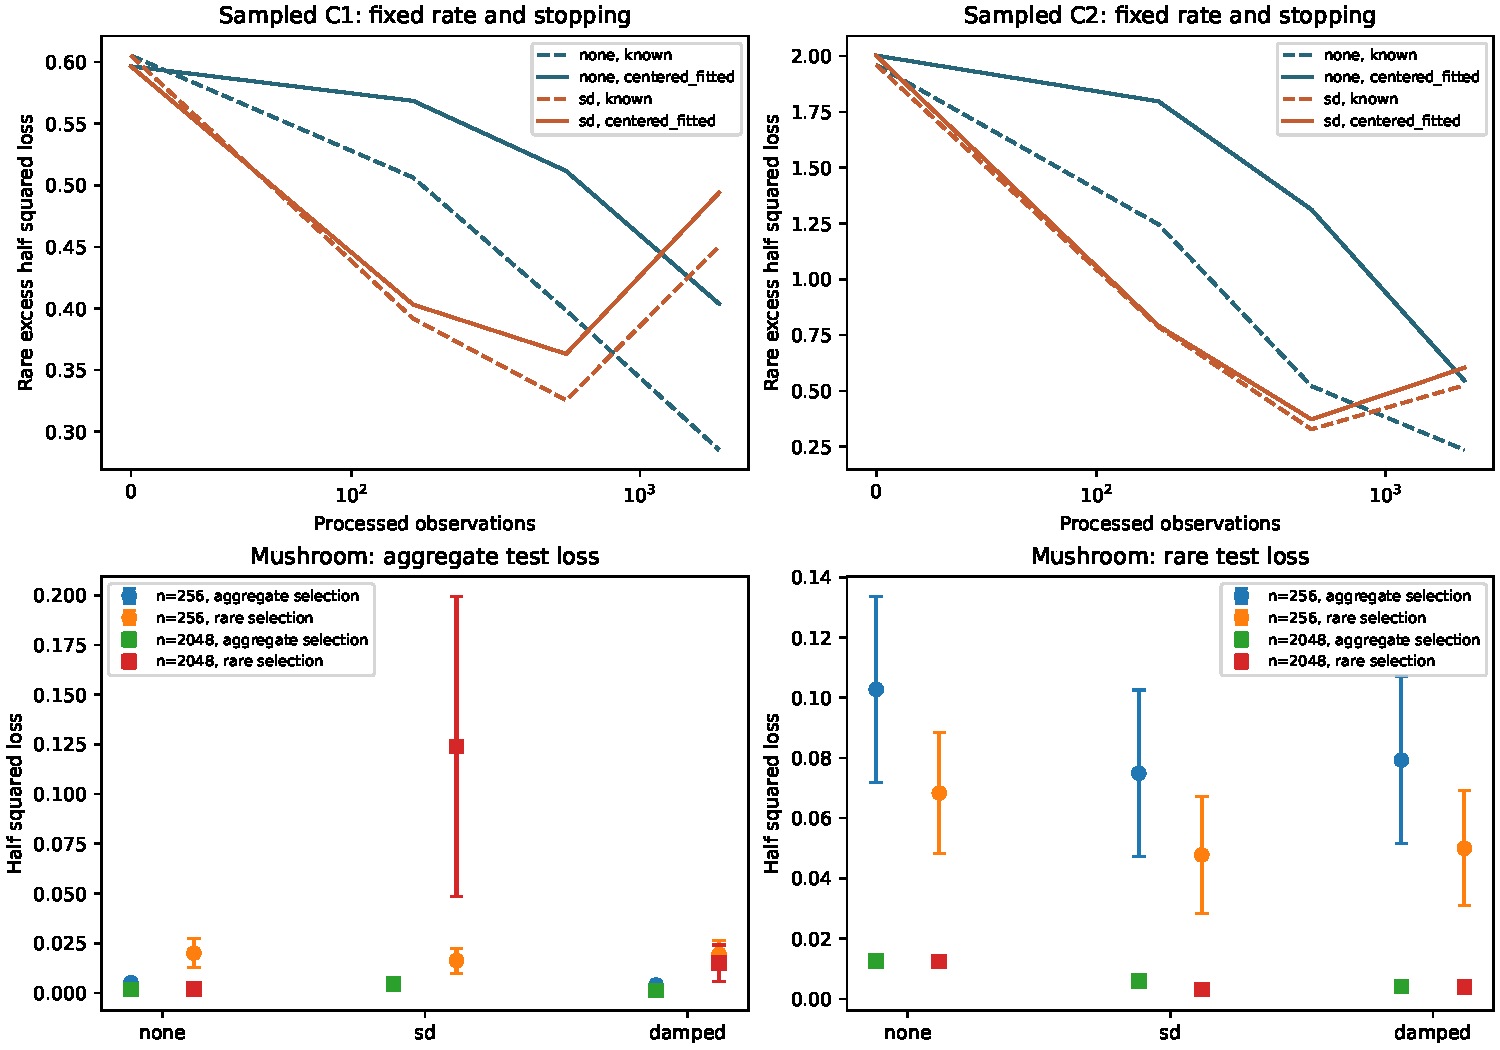
\includegraphics[width=\textwidth]{../results/practical-selection/practical-selection.pdf}
\caption{Practical normalization comparisons from the frozen sampled-data
study. Top: fixed-configuration paths for the independent and dependent
anchor laws under known preprocessing and training centering with a fitted
intercept. These use empirical rate calibration, not the theorems' fixed
$h$. Bottom: Mushroom held-out risks under aggregate and rare validation
selection at both sample sizes. Error bars show one Monte Carlo standard
error across replications or partitions; they are not population confidence
intervals for the Mushroom source.}
\label{fig:conference-practical}
\end{figure*}

\paragraph{When validation contains no rare cases.}
At $q=.002$, the two anchor laws have empty rare validation groups in
106 and 105 of 128 replications. The declared rare-selection rule falls
back to aggregate loss in those cases. One selected centered SD fit has
rare coefficient about $-6.719\times10^{16}$ and validation half squared
loss $2.086$, but exact-cell rare loss about $2.257\times10^{33}$.
A 160-digit decimal replay of all eligible trajectories in the worst
selected replication of each of 24 law/scaling panels leaves all 24
selections unchanged. The failure is not explained by detected
floating-point cancellation. Extreme finite outcomes and 151 failed
synthetic endpoints remain in the archive; tail-dominated means are not
precise population-risk estimates.

\subsection{A sparse categorical prediction task}

We predict the recorded poisonous label in UCI Mushroom
\citep{uciMushroom} using squared loss and all 22 categorical predictors.
The declared subgroup is green spore-print color: 72 of 8124 records.
Training data alone determine the one-hot vocabulary, means, and scales.
Missingness is a category and unknown categories map to zero blocks.
The design uses sparse storage and algebraic centering. Coefficients are
reported on the original feature scale; in the rank-deficient full
one-hot design, they are optimizer-dependent rather than uniquely
identified effects. Predictions are not clipped.

We use 32 random partitions at each training/validation size $(256,128)$
and $(2048,1024)$, with remaining records reserved for testing. Candidates
share partitions and replacement index streams. Each scaling receives the
same five rate factors and $B\in\{16,128\}$, with
$M\in\{512,2048,8192\}$. Table~\ref{tab:conference-mushroom} reports the
largest sample and cap with joint rate, batch, and stopping selection.

\begin{table}[t]
\centering
\begin{tabular}{llrr}
\toprule
Selection & Scaling & Aggregate & Rare \\
\midrule
Aggregate & None & .001754 & .012482 \\
 & SD & .004617 & .005912 \\
 & Damped & .001175 & .004151 \\
Rare & None & .001878 & .012465 \\
 & SD & .123905 & .003158 \\
 & Damped & .014966 & .003984 \\
\bottomrule
\end{tabular}
\caption{Mean held-out half squared loss for Mushroom, with $n=2048$,
1024 validation records, a fitted intercept, and cap $M=8192$.
Each scaling receives ten trajectories. Paired uncertainty is reported
in the text; marginal MCSEs appear in Appendix~\ref{sec:practical}.}
\label{tab:conference-mushroom}
\end{table}

Under aggregate selection, the SD-minus-none rare gap is $-.00657$
(paired MCSE $.00153$), with aggregate gap $+.002863$ ($.00213$).
Selecting SD by rare loss instead reduces its rare loss by $.002754$
($.000967$), with a variable aggregate penalty of $.11929$ ($.0756$).
The mean green coefficient under aggregate selection is $.4822$ for
none, $.7462$ for SD, and $.7678$ for damped scaling. Other coefficients
partly offset this larger contribution to rare predictions.

The result is conditional on the declared search. All 32 large-sample
unscaled aggregate selections choose the largest rate factor, so its
continuous optimum is unresolved. The small-sample experiment has no
green training observations in five partitions and none in validation
in thirteen. MCSEs describe partition and optimization variation within
this dataset. The source comprises hypothetical descriptions derived
from a field guide, so random-record performance does not establish
generalization to new species or field data.
